\documentclass[a4paper,12pt,draft]{article}
\usepackage{a4wide}
\usepackage{ucs}
\usepackage[utf8x]{inputenc}
\usepackage{subfigure}
\usepackage{xcolor}
\usepackage[czech]{babel}
\usepackage[pdftex, final]{graphicx}
\usepackage[pdftex, final, colorlinks=true]{hyperref}
\usepackage{verbatim}
\usepackage{mdwlist}
\parskip=0.8ex plus 0.4ex minus 0.1 ex


%%%%%%%%%%%%%%%%%%%%%%%%%%%%%%%
\usepackage[final]{listings}

\definecolor{lightGrey}{RGB}{250,250,250}
\definecolor{darkGrey}{RGB}{100,100,100}
\lstdefinelanguage{psmap}
{morekeywords={scale, mapinfo, maploc, where, end, font, fontsize, color, border, raster, width, paper,
vpoints, vareas, vlines, symbol, size, rgbcolumn, sizecolumn, cwidth, rotatecolumn, },
morekeywords=[2]{y, n, none},
morecomment=[l]{\#},
}
\lstdefinestyle{psmap}{
   language=psmap,
   basicstyle={\sffamily},
   keywordstyle=[1]{\bfseries},
   keywordstyle=[2]{\color{darkGrey}},
   commentstyle={\itshape},
   frame=lines,
   backgroundcolor=\color{lightGrey},
}
\lstdefinestyle{psmapInline}{
   language=psmap,
   basicstyle={\sffamily},
   keywordstyle=[1]{},
   keywordstyle=[2]{\bfseries\color{darkGrey}},
   commentstyle={\itshape},
   frame=lines,
   backgroundcolor=\color{lightGrey},
}
\lstnewenvironment{psmap}[1][]
{\lstset{style=psmap,
   #1}}
   {}

\newcommand{\modul}[1]{\emph{#1}}
\newcommand{\instr}[1]{\lstinline[style=psmapInline]|#1|}
\author{Anna Kratochvílová}


\begin{document}
\tableofcontents
\section{Úvod}

\section{Tvorba mapových výstupů}

\subsection{Porovnání možností programů pro tvorbu mapových výstupů}

\subsubsection{ArcGIS}

\subsubsection{QGis}

\subsubsection{gvSIG}

\subsubsection{GRASS GIS -- ps.map}
\label{sec:porovnani:psmap}

\section{Zásady tvorby grafického uživatelského rozhraní}
\subsection{Čeho se vyvarovat}
\subsection{Co je vhodné}


\section{Systém GRASS GIS}

\subsection{Grafické rozhraní systému GRASS GIS}

\subsection{Modul ps.map}
\label{sec:psmap}
Modul \modul{ps.map} lze jako většinu modulů používat z příkazové řádky GRASSu nebo pro\-střed\-nic\-tvím wxGUI. Grafické rozhraní je vytvořeno stejným způsobem jako u většiny ostatních modulů, dovoluje tedy zadat parametry příkazu v dialogu. V tomto případě ale spouštění přes grafické rozhraní neskýtá mimořádnou výhodu, jelikož v zásadě většinou stačí zadat jméno již připraveného konfiguračního souboru a souboru výstupního, což je pro mnohé uživatele pohodlnější prostřednictvím příkazové řádky. V příkazové řádce vypadá spuštění \modul{ps.map} takto:
\begin{verbatim}
 ps.map input=/konfiguracni/soubor.txt output=/vystupni/soubor.ps   
\end{verbatim}

Jak již bylo zmíněno v části \ref{sec:porovnani:psmap}, modul vytváří mapový výstup na základě konfiguračního souboru, což je obyčejný textový soubor s instrukcemi. Vytvořit tento soubor je většinou poměrně pracné, umisťování mapových prvků na vhodnou pozici se často neobejde bez vedlejších výpočtů, což ke konformitě používání příliš nepřispívá. Z toho je zřejmé, že v současnosti \modul{ps.map} využívá pouze poměrně úzká komunita uživatelů GRASSu. Nové grafické rozhraní přímo vytváří konfigurační soubor, na základě něhož poté \modul{ps.map} vygeneruje mapový výstup. Není pak třeba se konfiguračním souborem zabývat, což může zpříjemnit používání tohoto modulu, a tím i rozšířit řady jeho uživatelů. 

\subsubsection{Konfigurační soubor}
Konfigurační soubor má poměrně jednoduchou strukturu. Skládá se z instrukcí, které musí být na samostatných řádcích. Instrukce mohou obsahovat další dílčí instrukce umístěné opět na samostatných řádcích. Tyto víceřádkové instrukce musí být ukončeny  instrukcí \instr{end}, která musí být uvedena i na konci celého konfiguračního souboru. Dílčí instrukce je možné ve většině případů vynechat a pro nastavení dané vlastnosti se použije implicitní hodnota. Komentáře lze zapisovat pomocí znaku \#, prázdné řádky jsou ignorovány. Pořadí instrukcí většinou nehraje roli s výjimkou instrukcí \instr{vpoints}, \instr{vlines} a \instr{vareas}, které vykreslují vektorové vrstvy. První uvedená vektorová vrstva bude vykreslena nejvýše. Více napoví ukázka jednoduchého konfiguračního souboru:
\begin{psmap}
paper a3
end
raster soils            # priklad jednoradkove instrukce
border y                # priklad viceradkove instrukce ...
   color 255:0:0
   width 3
end                     # ... ukoncene instrukci end
vpoints archsites
   symbol basic/diamond
   size 10
end
end                     # konec instrukci
\end{psmap}
Význam jednotlivých instrukcí je popsán v manuálové stránce k modulu, která je dostupná buď z dosavadního GUI nebo na internetových stránkách \cite{manual}.

\subsubsection{Volba rozsahu zobrazovaného území}
\label{sec:psmap:rozsah}
V konfiguračním souboru lze nastavit velikost mapového okna, čímž je myšlen obdélník s vykreslenou rastrovou či vektorovou mapou.  K nastavení slouží jednořádková instrukce \instr{maploc}, která umístí levý horní roh okna na dané místo a volitelně nastaví i šířku a výšku mapového okna. Rozměry lze nepřímo ovlivnit také instrukcí \instr{scale}, která na základě měřítka upraví rozměry okna. 

Nicméně při jakýchkoli rozměrech a umístění mapového okna, se vykresluje stále stejný územní rozsah. Ten je dán tzv. \emph{výpočetním regionem}. Proto je třeba před vlastním generováním mapového výstupu nastavit výpočetní region tak, aby odpovídal území, které chceme zobrazit. K tomu slouží modul \modul{g.region}. V konfiguračním souboru tedy nelze rozsah území ovlivnit.
Modul \modul{ps.map} tedy nejprve zjistí požadované rozměry a měřítko z konfiguračního souboru (jsou-li uvedeny) a následně se je pokusí aplikovat na rozměry současného výpočetního regionu. Když by se mapové okno při požadovaném měřítku nevešlo na daný formát papíru, modul měřítko upraví. Podobně upraví rozměry mapového okna, aby se vešlo do zadaných rozměrů.

Nové grafické rozhraní \modul{ps.map} řeší volbu zobrazovaného území ve vlastní režii, není tedy třeba volat modul \modul{g.region} a zároveň se nemění současný výpočetní region pro ostatí moduly. %Více v oddíle 

\subsubsection{Nekonzistence a chyby v modulu ps.map}
\label{sec:psmap:chyby}
Při tvorbě grafického rozhraní bylo nutné prozkoumat chování modulu \modul{ps.map} o něco detailněji, než je nutné pro jeho běžné užívání. Vycházela jsem především z manuálové stránky \cite{manual} a vlastního experimentování s modulem. 

\paragraph*{Souřadnicové systémy a jednotky}
\label{sec:psmap:sour_systemy}
Jedním z nejnepříjemnějších problémů, se kterými bylo třeba se při tvorbě GUI vypořádat, byla nekonzistence v jednotkách a souřadnicových sytémech. Modul \modul{ps.map} totiž pro umístění jednotlivých prvků (jako legenda, text, měřítko) používá dva různé systémy, viz obr. č. \ref{fig:sour_systemy}.

\begin{figure}[h!]
    \centering
    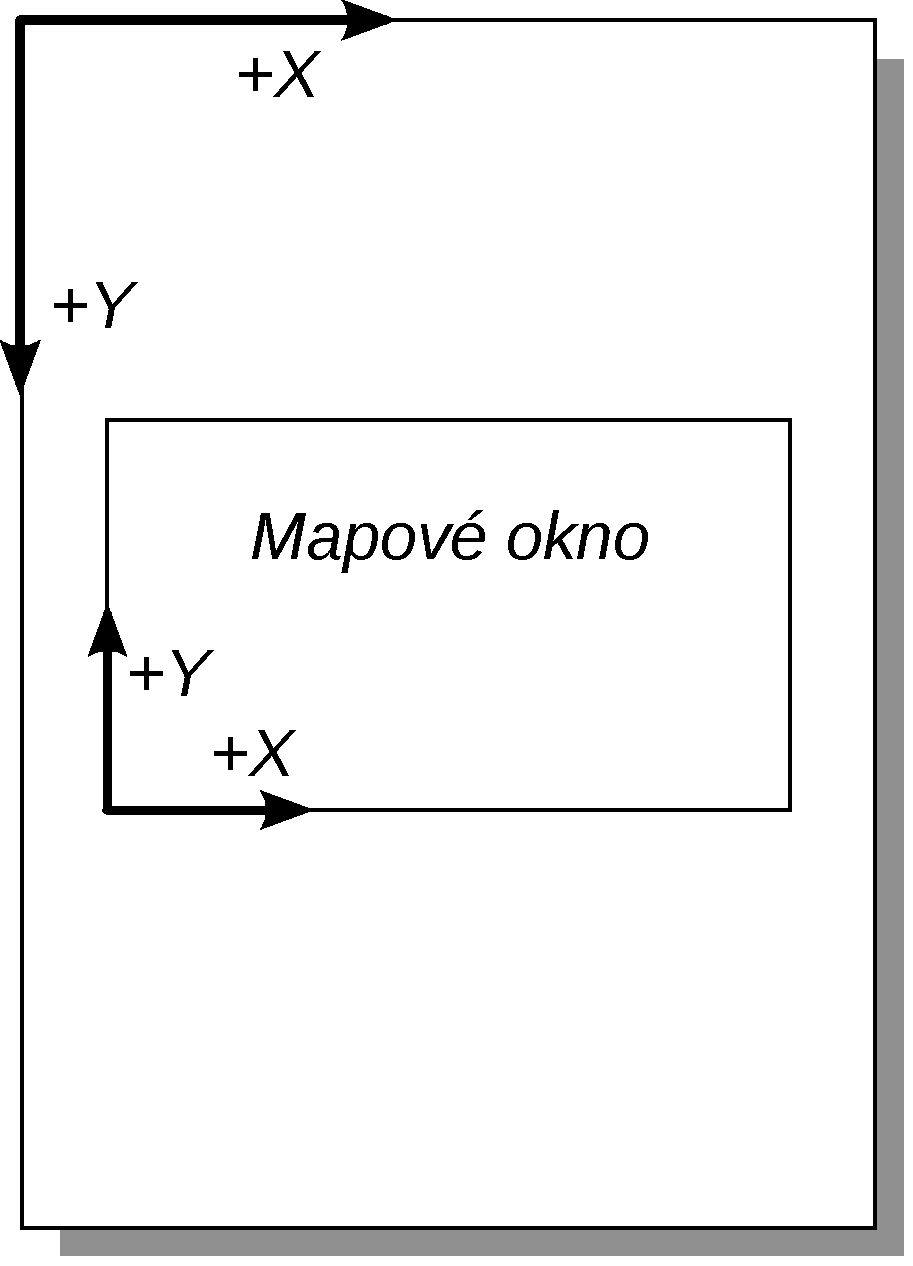
\includegraphics[width=0.2\textheight]{./sour_systemy.pdf}
    \caption{Souřadnicové systémy používané modulem \modul{ps.map}\label{fig:sour_systemy}}
\end{figure}


První z nich -- souřadnicový systém papíru -- má počátek v levém horním rohu, kladná osa \emph{x} směřuje doprava a osa \emph{y} směrem dolů (tedy odpovídá systému obvyklému v počítačové grafice). 
Je-li poloha určena v tomto sytému, očekávanou jednotkou je inch\footnote{ česky palec, odpovídá $2{},54$ cm}.

Druhý systém -- systém mapového okna -- má počátek souřadnic v levém dolním rohu mapového okna s pravotočivou orientací os obvyklou v matematice. Souřadnice lze v tomto systému zadávat dvěma způsoby. Buď v procentech výpočetního regionu nebo přímo v souřadnicích mapy. Například, při souřadnicích [100\%, 0\%] je objekt umístěn v pravém dolním rohu mapového okna, ať už je mapové okno na papíře umístěno kdekoli. Alternativně bychom toho samého umístění dosáhli zadáním mapových souřadnic bodu položeného co nejvíce na východ a jih v rozsahu výpočetního regionu. Oběma způsoby lze dosáhnout i umístění objektu mimo mapové okno, a to zadáním záporné hodnoty nebo hodnoty větší než 100 u procent, případně mapových souřadnic mimo výpočetní region.

Různé způsoby určení polohy mají své opodstatnění. V některých případech je výhodné umístit popisek k určitému místu, jehož mapové souřadnice známe, a jeho poloha vzhledem k papíru není podstatná. Pozicování pomocí procent je vhodné například pro nadpis mapy, který chceme umístit přesně doprostřed nad mapové okno. 

Problém nastává v případě, když chce uživatel určit polohu objektu relativně k papíru a tento objekt podporuje umístění pouze relativně k mapovému oknu, případně naopak. Bylo by proto vhodné, aby všechny objekty podporovaly umístění všemi těmito způsoby. Uživatel by si pak mohl vybrat, který z nich je pro danou situaci nejvhodnější.

\paragraph*{Referenční bod objektu}
\label{sec:psmap:referencepoint}
Modul \modul{ps.map} u většiny objektů nepodporuje volbu referenčního bodu, tedy bodu objektu, ke kterému se vztahuje zadaná poloha. Výjimkou je text, u nějž si lze vybrat jeden z devíti referenčních bodů. Je zřejmé, že u textu má tato volba smysl, u ostatních objektů je otázka, zda by tato vlastnost byla využívaná. 
U ostatních objektů je referenční bod dán a nelze měnit. Uživatele však může překvapit, že není u všech objektů stejný. Ve většině případů se poloha vztahuje k levému hornímu rohu objektu, nicméně grafické měřítko (instrukce \instr{scalebar}) má referenční bod ve středu. Bylo by vhodné tento přístup sjednotit, na druhou stranu nejde o nijak zásadní problém. 

\paragraph*{Volba barev}
\label{sec:psmap:color}
V mnoha instrukcích se vyskytuje nastavení barvy. Bohužel velká část instrukcí omezuje výběr barev tím, že vyžaduje zadat barvu ve formě jejího jména, tedy např. \emph{aqua}, \emph{black}, \emph{blue}, \ldots Některé jiné instrukce však umožňují zadat barvu i ve tvaru R:G:B. Bylo by proto logické, kdyby RGB podporovaly všechny instrukce.

\paragraph*{Jednořádkové a víceřádkové instrukce}
\label{sec:psmap:singleline}
Instrukce \instr{border} (ohraničení mapového okna) a \instr{colortable} (rastrová legenda) mohou být jednořádkové i víceřádkové, což mimo jiné znamená, že někdy je \instr{end} za příkazem vyžadováno a někdy naopak následovat nesmí. Záleží, zda za zmíněné instrukce do stejného řádku napíšeme \instr{y} nebo \instr{n}, tím ji lze zapnout a vypnout. 
\begin{psmap}
border n    # jednoradkova instrukce - nesmi nasledovat end

border y    # viceradkova instrukce - musi nasledovat end
   width 2
end
\end{psmap}
Je nepříjemné, že si uživatel musí být vědom tohoto chování, jinak by se mu mohlo snadno stát, že napíše instrukci \instr{end}, kde být nemá, a \modul{ps.map} to bude považovat za konec souboru a další instrukce bude ignorovat.
Navíc u \instr{colortable} nemá možnost zapínání a vypínání valného smyslu, když tuto instrukci neuvedu, legenda se prostě nevykreslí.

\paragraph*{Mapinfo}
\label{sec:psmap:mapinfo}
Mapový prvek \emph{mapinfo}, se v některých případech špatně vykreslí. Problém nastává, když jej uživatel chce umístit nalevo od mapového okna. Modul \modul{ps.map} přesune mapinfo tak, že se vertikálně zarovná k mapovému oknu, neboli převezme \emph{x}-ovou sořadnici okna. Další chybou je špatné barevné vykreslení barvy pozadí a ohraničující linie. Barvy se nevykreslí, když je mapinfo  mimo mapové okno. 

\paragraph*{Nekonzistence u instrukce \instr{vlines}}
\label{sec:psmap:vlines}
U instrukce \instr{vlines} která přidává liniovou vektorovou vrstvu, lze použít dílčí instrukci \instr{rgbcolumn}. Ta vykreslí   linii barvou uvedenou ve zvoleném sloupci atributové tabulky na příslušném řádku. Podobně lze použít dílčí instrukci \instr{cwidth}, která ovlivňuje šířku vykreslené linie. Šířka je pak určena zadanou hodnotou pronásobenou číslem kategorie (sloupec \emph{cat} v atributové tabulce), do níž linie patří. V tomto případě si tedy uživatel nemůže zvolit, podle jakého atributu se bude šířka řídit, což v prvním případě jde. Bylo by vhodné tento přístup sjednotit. 

\paragraph*{Nepřesnosti v dokumentaci}
\label{sec:psmap:manual}
Manuálová stránka \cite{manual} k modulu \modul{ps.map} je poměrně podrobná a vyčerpávající, přesto lze narazit na některé nepřesnosti. Například u instrukce \instr{text} je k popisu dílčí instrukce \instr{width} napsáno:
 \begin{quotation}\it
width of the lines used to draw the text to make thicker letters
\end{quotation}
Prakticky však tato instrukce ovlivňuje šířku rámečku kolem textu.

Popis instrukce \instr{colortable} (vytváří rastrovou legendu) je místy matoucí. Jsou totiž dva typy rastrové legendy, což záleží na typu dat (\emph{CELL} -- celočíselný rastr a \emph{FCELL, DCELL} -- neceločíselný rastr). Některé dílčí instrukce mají pak smysl pouze pro jeden typ, případně se jejich význam pro jednotlivé typy liší. Situace se dále komplikuje dílčí instrukcí \instr{discrete}, která umožňuje změnit typ legendy. Manuál se sice snaží problematiku vysvětlit, ale ne příliš úspěšně, účinější je prakticky vše vyzkoušet.

\paragraph*{Orientace stránky}
Volbu orientace stránky zajišťuje přepínač \emph{-r} (rotate), který je-li uveden, mění orientaci stránky na šířku. Nevidím důvod, proč by se tato tato volba neměla provést již v konfiguračním souboru v rámci instrukce \instr{paper}, kam logicky patří. Význam by přepínač měl, kdybychom chtěli vytvořit ze stejného konfiguračního souboru výstupy s různou orientací stránky, to ale smysl příliš nedává.

\paragraph*{Titulek výstupního souboru}
Výstupní soubor má titulek \emph{Mapset = \textless aktuální mapset\textgreater}, což mnoho neříká a navíc rovnítko v titulku nepůsobí hezky. Uživatel by mohl mít možnost změnit titulek, případně by se titulek měl převzít z aktuálního rastru, případně vektoru\footnote{GUI aplikace by sice mohla napravit tento nedostatek, nicméně je vhodnější toto upravit přímo v modulu \modul{ps.map}.}.

\section{Grafické rozhraní pro modul \modul{ps.map}}
\label{sec:gui}

Důvody, proč je nové grafické rozhraní pro modul \modul{ps.map} zapotřebí, jsou zmíněny již v části \ref{sec:psmap}. Účelem je především oprostit uživatele od nutnosti ručně vytvářet konfigurační soubor. 

\subsection{Stažení programu z repozitáře add-ons}
% Aplikace je napsána primárně pro GRASS 7 a měla by fungovat i v GRASS 6.5. %a testována pod operačním systémem Linux, distribuce Ubuntu 10.04 LTS.
% Popíši postup pro GRASS 7. 
\subsection{Podklady a použité knihovny}
Nové grafické uživatelské rozhraní pro modul \modul{ps.map} bylo vyvinuto pomocí knihovny wxPython, 
proto bylo nutné se s knihovnou podrobněji seznámit. Jedním z nejvýznamnějších zdrojů informací je demo pro wxPython \cite{demo}, ve kterém je názorně ukázáno chování všech dostupných widgetů. Při hledání vhodného widgetu pro aplikaci je demo velice užitečné. 

Při psaní programu jsem pracovala s knihovnou \emph{GRASS Python Scripting Library} \cite{script}, která umožňuje a zjednodušuje volání modulů GRASSu. Zdrojem informací mi byly také již napsané GRASS wxGUI moduly. Seznámila jsem se také s moduly GRASSu, zjišťovala jsem především, co umožňují, a jak je mohu pro práci využít. 

\subsection{Funkcionalita aplikace}
V následujícím textu jsou shrnuty hlavní vlastnosti GUI aplikace a možnosti jejího využití.
\paragraph*{Podporované instrukce}
    Aplikace v současné době podporuje pouze vybrané instrukce, a to: \instr{border}, \instr{colortable}, \instr{mapinfo}, \instr{maploc}, \instr{paper}, \instr{raster}, \instr{scale}, \instr{scalebar}, \instr{text}, \instr{vareas}, \instr{vlines}, \instr{vpoints} a \instr{vlegend}. V budoucnu se počítá s podporou dalších instrukcí. Pokud uživatel potřebuje použít některé dosud nepodporované instrukce, má možnost část práce vykonat v GUI aplikaci a nechat si vygenerovat konfigurační soubor. Tam tyto instrukce doplní a spustí přímo modul \modul{ps.map}.
\paragraph*{Možné výstupy aplikace}
Výsledkem práce s GUI aplikací je mapový výstup ve formátu PostScript, případně Encapsulated PostScript, který je vygenerován modulem \modul{ps.map} na základě konfiguračního souboru vytvořeném GUI aplikací. Dalším možným výstupem je konfigurační soubor samotný, který lze dále zpracovávat.

\paragraph*{Čtení konfiguračních souborů}
Aplikace umožňuje také konfigurační soubory načítat. Vhodnější je ale načítat soubor vytvořený touto aplikací. To dáno tím, že aplikace při vytváření konfiguračního souboru zapisuje i informace o regionu do komentáře, což není standardní součástí konfiguračního souboru. Navíc je aplikace více otestovaná právě pro načítání vlastních souborů\footnote{Je nutné podotknout, že si aplikace nevytváří žádný vlastní odlišný formát.}. 

\paragraph*{Koncept a náhled}
Aplikace rozlišuje dva módy -- koncept a náhled (\emph{Draft mode} a \emph{Preview mode}). 
Uživatel vytváří mapový výstup v módu konceptu, což znamená, že jednotlivé vykreslované prvky jako legenda či mapové okno jsou představovány pouze barevným obdélníkem s popisem typu objektu. Jejich vzhled tedy nijak nesouvisí se jejich skutečným vykreslením modulem \modul{ps.map}, s výjimkou jejich rozměrů. Ty odpovídají rozměrům skutečným (alespoň se o to snaží, viz část \nameref{sec:gui:problemy}). Objekty lze posunovat po papíře, s výjimkou mapového okna však nelze měnit jejich rozměry.
Při práci lze průběžně kontrolovat výsledek pomocí módu náhledu. Na pozadí je spuštěn modul \modul{ps.map}, který vygeneruje dočasný PostScript soubor, ten je překonvertován do PNG a zobrazen v GUI aplikaci. To vše samozřejmě zabere poměrně dost času, záleží na složitosti mapového výstupu. Konverze do PNG je také poměrně časově náročná. Proto může být lepší si vygenerovat přímo PS soubor a ten si zobrazit v externím prohlížeči.
% dvě roviny, vykresleni v GUI a vykreslení skutečné

\subsection{Základní práce s GUI aplikací}
% Práce s GUI vypadá tak, že uživatel na stránku umístí zvolené mapové prvky, provede nastavení jejich vlastností v dialozích a nechá si vykreslit výsledek. Program na základě zvolených nastavení vytvoří konfigurační soubor, se kterým poté spustí modul \modul{ps.map}. Výstupem může být konfigurační soubor, PS soubor (případně EPS) a výsledek je viditelný i přímo v GUI.

\subsection[Problémy při tvorbě GUI]{Problémy při tvorbě GUI pro \modul{ps.map} a jejich řešení}
\label{sec:gui:problemy}
Při práci jsem narazila na několik problematických oblastí, které se částečně kryjí se záležitostmi popsanými v části \ref{sec:psmap:rozsah} a \ref{sec:psmap:chyby}. 

\paragraph*{Výpočetní region} Připomeňme, že modul \modul{ps.map} pracuje s aktuálním výpočetním regionem a vykresluje mapy pouze v tomto rozsahu. Jelikož by bylo nepohodlné, kdyby uživatel musel při práci v novém \modul{ps.map} GUI nastavovat region externě pomocí GRASS modulu \modul{g.region}, je vše řešeno v rámci této aplikace. Uživatel si v aplikaci určitým způsobem nastaví region, který pak \modul{ps.map} použije k zobrazení. Stávající výpočetní region, který mezitím mohou používat další moduly GRASSu, zůstane nezměněný. Když si uživatel nechá vygenerovat konfigurační soubor, který chce dále editovat ručně, je v záhlaví v komentáři napsán příkaz pro modul \modul{g.region}, který informuje o výpočetním regionu nastaveném v době vzniku souboru. Tato informace se využívá i při čtení konfiguračního souboru vytvořeného touto aplikací.  Způsoby nastavení regionu jsou následující:
\begin{enumerate*}
    \item nastavit region na zvolenou rastrovou či vektorovou mapu
    \item nastavit uložený region (\emph{named region})
    \item nastavit aktuální výpočetní region
    \item zvolit souřadnice středu mapy a měřítko (nastavení regionu se automaticky vypočítá)
\end{enumerate*}


\paragraph*{Souřadnicové systémy a jednotky} Nepříjemným problémem byly používané souřadnicové systémy a jednotky (viz část \ref{sec:psmap:sour_systemy} na straně \pageref{sec:psmap:sour_systemy}).
 Jelikož interaktivní umisťování objektů na stránce je jednou hlavních výhod grafického rozhraní, bylo nutné problém nejednotností systémů a jednotek řešit vlastními přepočty v programu tak, aby byl od něj uživatel co nejvíce odstíněn. Na druhou stranu by bylo logičtější, aby potřebné výpočty prováděl už samotný modul \modul{ps.map}, který stejně už podobné výpočty provádí, stačilo by je pouze rozšířit. V důsledku toho se zřejmě určité výpočty provádí dvakrát -- v \modul{ps.map} a v GUI.
 
 GUI aplikace je navržená tak, aby polohu objektů uživatel určil interaktivně kliknutím na objekt a táhnutím myší. Navíc lze v dialozích k objektům zadat přímo \emph{x}-ovou a \emph{y}-ovou souřadnici v systému papíru. Zde jsem rozšířila stávající možnosti \modul{ps.map} o možnost zadat hodnoty v dalších jednotkách (mm, cm).  U textového objektu, který se zadává v druhém systému (tedy mapové souřadnice či procenta region), jsou uživateli nabídnuty možnosti dvě. Buď zadat souřadnice v systému papíru, nebo pomocí mapových souřadnic. Možnost zadání procent regionu GUI aplikace zatím nepodporuje, myslím, že tato možnost není již tak potřebná, když lze polohu měnit jednoduchým tahem myší. 
 
 \paragraph*{Referenční bod objektu} 
 Grafické měřítko má referenční bod ve svém středu, narozdíl od ostatních objektů, u kterých je to levý horní roh, viz \ref{sec:psmap:referencepoint}. Rozhodla jsem se přístup sjednotit, proto GUI aplikace provádí drobný přepočet a pokud uživatel zadává ručně souřadnice, vztahují se k hornímu levému rohu. V dialogu je tato skutečnost uvedena, aby uživatelé zvyklí na původní ref. bod nebyli zmateni.
 
 U textového objektu bylo řešení situace složitější. Zachovávám možnost zvolit si u textu jeho referenční bod, což znamená problémy při jeho zobrazování v GUI aplikaci. Situaci totiž komplikují další faktory jako rotace textu a odsazení (\emph{offset}).
 Gui aplikace by musela na základě těchto parametrů provádět zbytečně složité výpočty, aby byla schopna určit přesné místo, kam se má text vykreslit a jaký je jeho ohraničující obdélník. V tomto místě jsem narazila na určité rezervy, které knihovna \emph{wxPython} má. Očekávala jsem, že mi tyto výpočty knihovna aspoň částečně zjednodušší, ale jelikož jsem potřebné metody nenalezla, provedla jsem při výpočtech drobná zanedbání. Zobrazení v GUI aplikaci proto v některých případech není úplně přesné, nicméně je nutné zdůraznit, že to nijak nesouvisí se zobrazením textu ve  vygenerovaném souboru.
 
 \paragraph*{Tvorba dialogů}
 Každý mapový prvek jako např. mapinfo, grafické měřítko či legenda mají vlastní dialog, kde se nastavují jejich vlastnosti. Dialogy jsou různě rozsáhlé, ale mají podobný vzhled. Problém při tvorbě dialogů byla celková nejednotnost v nastavitelných vlastnostech dialogů. Například, rastrová legenda umožňuje změnit barvu písma a neumožňuje vykreslit ohraničení (\emph{border}), zatímco u vektorové legendy je to přesně naopak. Takových případů je víc a značně komplikují snahy o ujednocení vzhledu dialogů. Proto by bylo příliš náročné vytvořit jakýsi jednotný dialog pro nastavení vlastností objektů, pravděpodobně by to vedlo k větší nepřehlednosti. 
 
 

\subsection{Ukázky}

\section{Závěr}

\begin{thebibliography}{9}
\label{literatura}
\bibitem{manual} GRASS Development Team. \textit{GRASS GIS 7.0.svn Reference Manual} [online], c2003-2011 [cit. 2011-03-19].\\ URL: \url{http://grass.fbk.eu/grass70/manuals/html70_user/ps.map.html}
\bibitem{script} GRASS Development Team. \textit{GRASS 7 Programmer's Manual} [online], c2000-2011 [cit. 2011-03-19].\\ URL: \url{http://grass.osgeo.org/programming7/}
\bibitem{demo} Robin Dunn and Total Control Software. \textit{wxPython demo} [program], c1997-2006 [cit. 2011-03-19].\\ URL: \url{http://downloads.sourceforge.net/wxpython/wxPython-demo-2.8.11.0.tar.bz2}
\end{thebibliography}
\end{document}



